% vim:ft=tex

\section{General}
The Pelias API and Pelias services are only suited for the purpose of geocoding and reverse geocoding. Geocoding retrieves coordinates (latitude and longitude) for a given address or postode and reverse geocoding finds the nearest known address or postcode for a provided pair of latitude and longitude.
In order to find the shortest or fastest route between two given addresses Pelias has to be used in conjunction with a routing engine. The two addresses are fed into Pelias and Pelias provides coordinates for them which are then used as input values for finding a route from one coordinate to the other using a routing engine and the metrics inside the routing engine.
The senior team used the routing engine Graphhopper in connection with their geocoding service Nominatim. Graphhopper as you will see later in this report is a very good and fast routing engine, however the developers of the Pelias service recommend using the routing engine Valhalla which is developed by the same company (Mapzen) as Pelias and therefore has better service interoperability with Pelias than any other routing engine.
\subsection{Comparison of Routing Engines}
Part of this project was to research and evaluate possible routing engines for Pelias. Internet research conducted by the junior them revealed a comparison of open source routing engines which was done by one of the members of Openstreetmaps. The following two figures illustrate the required computing time (in ms) to calculate a route depending on the length of the route (in km)\citep{Ramm2017}:
\begin{figure}[H]
\centering
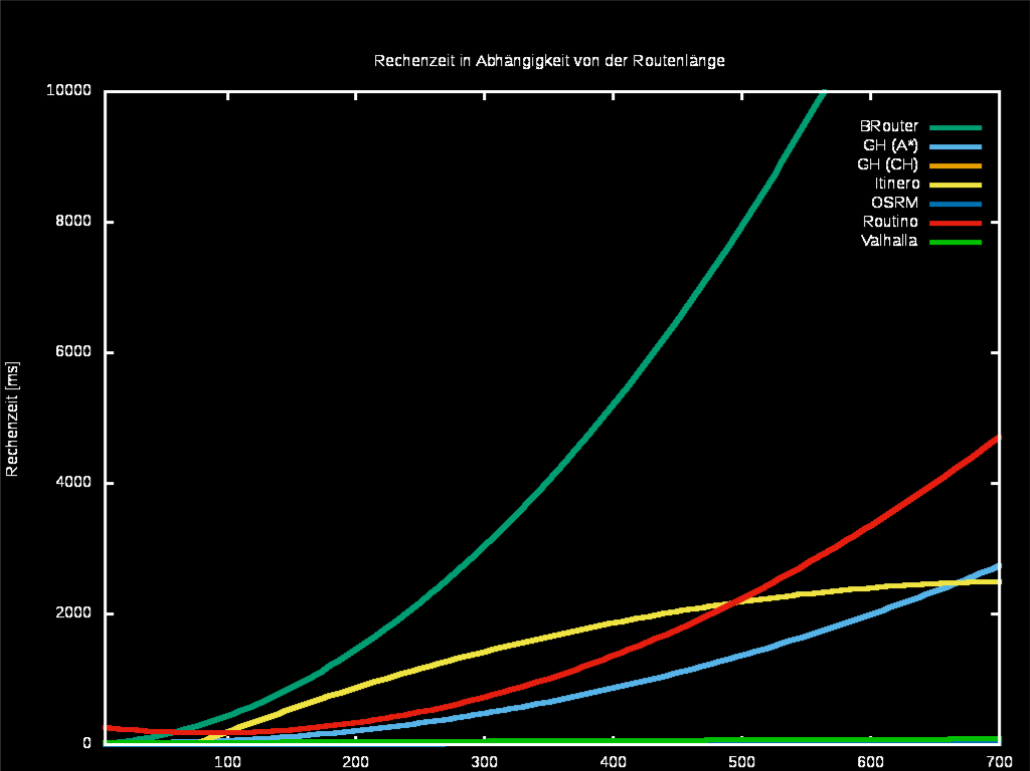
\includegraphics[width=1.0\textwidth]{img/routing_comparison_01}
\captionof{figure}{Comparison of all open source Routing Engines}\label{fig:routing_comparison_01}
\end{figure}
\begin{figure}[H]
\centering
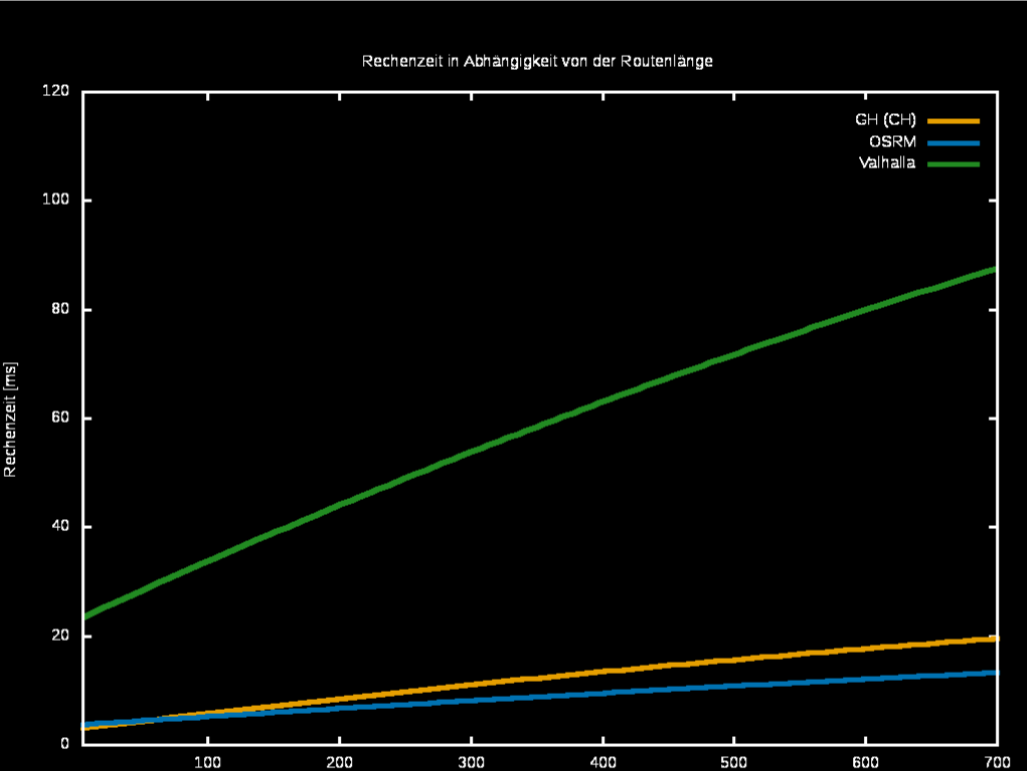
\includegraphics[width=1.0\textwidth]{img/routing_comparison_02}
\captionof{figure}{Comparison of fastest open source Routing Engines}\label{fig:routing_comparison_02}
\end{figure}
As can be seen, Graphopper (GH), Open Source Routing Machine (OSRM) and Valhalla are the best-performing open source routing engines. Therefore, a closer look can be taken at those three in the table \ref{CoRE}.
%
\begin{longtable}{|p{3.0cm}|p{3.0cm}|p{3.0cm}|p{3.0cm}|}
\caption{Comparison of Routing Engines \label{CoRE}}\\ \hline
\textbf{Comparison Criteria} & \textbf{Graphhopper} & \textbf{Valhalla} & \textbf{OSRM} \\ \hline
\endfirsthead
\caption{Comparison of Routing Engines (Continued)} \\ \hline
\textbf{Comparison Criteria} & \textbf{Graphhopper} & \textbf{Valhalla} & \textbf{OSRM} \\ \hline
\endhead
\multicolumn{4}{|r|}{Continued on next page}\\ \hline
\endfoot
\hline
%
\endlastfoot
\textbf{License} & Apache-License (proprietary in parts) & MIT license & BSD license \\ \hline
\textbf{OS} & Java (also Android, iOS) & C++, Apple/Linux & C++ (NodeJS), Apple/Linux/Windows \\ \hline
\textbf{Algorithm} & Contraction Hierarchies, Dijkstra/A*, Hybrid & A* with individual improvements & Contraction Hierarchies \\ \hline
\textbf{Documentation \& Setup} & Good documentation, ‘quick start’ & Good documentation, ‘quick start’, ubuntu repository with web-frontend & Good documentation, setup with docker or self-compiled \\ \hline
\textbf{Routing-features} & Turn restriction (A*), guidepost, alternatives, height data optional & Turn restriction, guidepost, height data optional & Turn restriction (A*), driving lanes, guidepost, alternatives, no height data \\ \hline
\textbf{Special Features} & Track Matching, cost != time, TSP with jsprit & Tile-based data storage, dynamic cost, matrix, isochrones, intermodal, Designed for working with OpenStreetMap & Matrix, track matching, TSP, data tiles, cost != time \\ \hline
\end{longtable}




Unfortunately OSRM has very high hardware requirements\citep{J.2017}. Preprocessing the car profile requires at least 175 GB of RAM and 280 GB of disk space. Additionally, 35 GB are needed for the planet osm.pbf (Openstreetmaps) and 40 to 50 GB for the generated data files. For the foot profile 248 GB of RAM are needed. During runtime the car profile requires around 64 GB of RAM, the foot profile even more. Basically OSRM loads the preprocessed files completely into RAM\citep{J.2017}. The project team's VM had only 64 GB of RAM and half of it was already used for Pelias and Elasticsearch. Hence, it was not possible to install OSRM and evaluate it completely.

\subsection{Graphopper vs Valhalla}
We performed an in-depth comparison of the time it takes for routing from one point to another with Graphhopper and Valhalla. The results of these test series can be seen in the table \ref{GHvsVH}.
%
\begin{longtable}{|p{0.5cm}|p{1.0cm}|p{2.0cm}|p{2.0cm}|p{2.0cm}|p{2.0cm}|p{2.0cm}|p{2.0cm}|}
\caption{Graphhopper vs. Valhalla test row \label{GHvsVH}}\\ \hline
                                       &                           & \textbf{Route 1} & \textbf{Route 2} & \textbf{Route 3} & \textbf{Route 4} & \textbf{Route 5} & \textbf{Route 6}  \\ \hline
\endfirsthead
\caption{Graphhopper vs. Valhalla test row (Continued)} \\ \hline
                                       &                           & \textbf{Route 1} & \textbf{Route 2} & \textbf{Route 3} & \textbf{Route 4} & \textbf{Route 5} & \textbf{Route 6}  \\ \hline
\endhead
\multicolumn{8}{|r|}{Continued on next page}\\ \hline
\endfoot
\hline
%\multicolumn{8}{|l|}{Graphhopper vs. Valhalla test row \label{GHvsVH}}\\ \hline
\endlastfoot
%\caption{Graphhopper vs. Valhalla test row \label{GHvsVH}}
                                       & \textbf{Route from}       & Catania, Italy Latitude: 37.502236 Longitude: 15.08738 & 1100-148 Lisbon, Portugal Latitude: 38.707751 Longitude: -9.136592 & Ulm, Baden-Württemberg, Germany Latitude: 48.3974 Longitude: 9.993434 & Paris, France Latitude: 48.856697 Longitude: 2.351462 & 37011 Bardolino VR, Italy Latitude: 45.553553 Longitude: 10.637519 & North Cape, E 69, Norway Latitude: 71.169951 Longitude: 25.785889 \\ \hline
                                       & \textbf{Route to}         &  1357 Copenhagen, Denmark Latitude: 55.686724 Longitude: 12.570072 & Warsaw, Warszawa, Poland Latitude: 52.231924 Longitude: 21.006727 & Munich, Bavaria, Germany Latitude: 48.137108 Longitude: 11.575382 & Venice, Venezia, Italy Latitude: 45.437191 Longitude: 12.33459 & Gunterstraße 8, 70191 Stuttgart, Germany Latitude: 48.806576 Longitude: 9.178105 & 89032 Bianco RC, Italy Latitude: 38.087176 Longitude: 16.148511 \\ \hline
\multirow{3}{*}{\textbf{GH}} & \textbf{first try}        & real 0m0.735s user 0m0.013s sys 0m0.006s & real 0m0.300s user 0m0.016s sys 0m0.006s & real 0m0.031s user 0m0.004s sys 0m0.011s & real 0m0.083s user 0m0.016s sys 0m0.000s & - & real 0m0.261s user 0m0.013s sys 0m0.011s \\ \hline
                                       & \textbf{sec-ond try}       & real 0m0.188s user 0m0.019s sys 0m0.000s & real 0m0.407s user 0m0.014s sys 0m0.005s & real 0m0.022s user 0m0.014s sys 0m0.000s & real 0m0.042s user 0m0.014s sys 0m0.004s & - & real 0m0.216s user 0m0.024s sys 0m0.004s \\ \hline
                                       & \textbf{dis-tance (in km)} & 2753 & 3318 & 139 & 1113 & - & 5112 \\ \hline
\multirow{3}{*}{\textbf{VH}}    & \textbf{first try}        & real 0m2.098s user 0m0.014s sys 0m0.013s & real 0m4.805s user 0m0.013s sys 0m0.021s & real 0m0.668s user 0m0.012s sys 0m0.006s & real 0m3.121s user 0m0.020s sys 0m0.003s & real 0m1.037s user 0m0.012s sys 0m0.009s & real 0m1.784s user 0m0.030s sys 0m0.003s \\ \hline
                                       & \textbf{sec-ond try}       & real 0m0.279s user 0m0.018s sys 0m0.008s & real 0m0.498s user 0m0.030s sys 0m0.003s & real 0m0.083s user 0m0.014s sys 0m0.004s & real 0m0.571s user 0m0.014s sys 0m0.008s & real 0m0.086s user 0m0.017s sys 0m0.005s & real 0m0.607s user 0m0.026s sys 0m0.008s \\ \hline
                                       & \textbf{dis-tance (in km)} & 2682 & 3408 & 141 & 1116 & 579 & 4996 \\ \hline
                                       & \textbf{re-mark}           &  &  &  &  & Coordinates of the starting point in the middle of lake garda. Graphhopper couldn’t calculate a route & 
\end{longtable}



The API requests were executed directly on the Graphhopper and Valhalla host machines using the command line programs time and curl.
We can see, that Graphhopper compared to Valhalla does a significantly better job when calculating a new route for the very first time. The execution time in Valhalla varies from the first calculation to the second calculation by up to the factor of ten. This means calculating a route or part of it, which has already been calculated before, the execution time is almost ten times faster compared to the first calculation. Valhalla achieves this with caching routes in RAM. Graphhopper however has a problem, if there is no road or street to be routed from or to for a given start- or end-point. Valhalla in this case just takes the closest routable point instead.  Choosing one routing engine over the other depends on the goal which should be achieved. For fastest execution time (not regarding first or second execution) Graphhopper fits best. If you want to make sure, that you receive a route whichever point you calculate from or to, then it is recommended to use Valhalla.

\subsection{Conclusion}
OSRM is the fastest routing engine on the open-source market. But because of the very high memory requirements of OSRM it is not suitable for the use-case of our project and the cost/benefit-factor is too low. Valhalla would be a good alternative to Graphhopper, because it is compared to other routing engines nearly as fast as Graphhopper and is designed to work with Openstreetmaps-data and also recommended by the Pelias developers to be used in connection with Pelias as a geocoder. Also Valhalla is capable of routing from or to points, which do not have a road or street directly nearby. A very valuable feature especially for two-digit postcode centroids, which Graphhopper does not have. However, in this early state of the project Graphhopper totally fits all the needs and therefore there is no need in replacing Graphhopper with Valhalla.

